\subsubsection{Setting The Heap Tree:}

To encode using the Huffman's algorithm we need to set a coding {\itshape tree} with the following conditions:

\begin{enumerate}
\item Set all the {\itshape symbols} in a priority queue according to its frequency.
\item Combine all the {\itshape symbol} less frequents in a single node of the tree.
\item Insert the new node to the priority queue.
\item Repeat steps 2 and 3 until there's only 1 element in the priority queue.
\end{enumerate} 

To create a priority queue in python we import the module {\bfseries heapq} that provides a priority queue based on heaps. Retaking the previously example, our priority queue shall look like in Figure 3.2.0. \hfill \break

\begin{figure}[H]
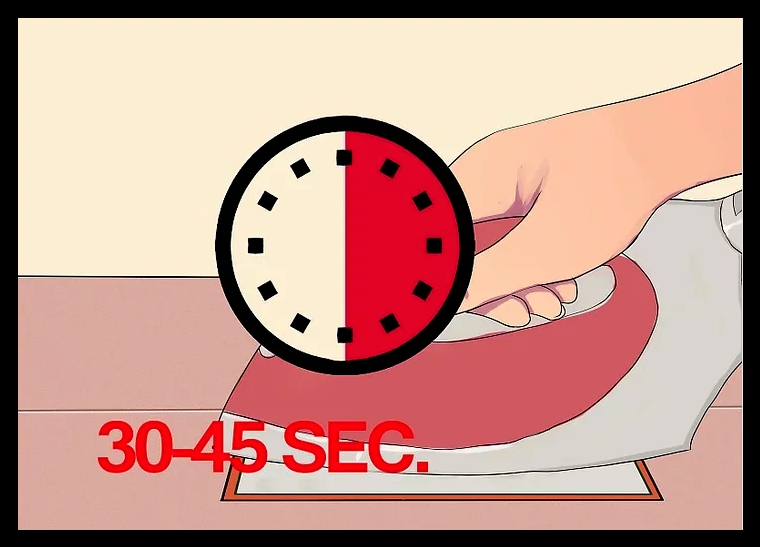
\includegraphics[height = 3cm, width = 16.5cm]{2.png}
\centering \linebreak \linebreak Figure 3.2.0: Priority queue for table's 1 column Frequency.
\end{figure} \hfill \break

The code works as follows, from the dictionary {\bfseries frequency} we extract each {\itshape symbol} with its {\itshape frequency}, then, in line 5 we append in the priority queue {\bfseries self.tree} as a tuple where its first element it's the frequency, the second it's the depth level on the {\itshape heap tree} that we will create later ( notice that as it is a priority queue, the depth level initially will be of "0" ) and the last element is the respective {\itshape symbol}, this should satisfied the step 1. From lines 7 - 12 we can find a {\bfseries while} loop, in lines 9 and 10 we {\bfseries pop} from the priority queue the less frequents {\itshape symbols}. In line 11 we create a new node that it's a {\itshape tuple} that stores the in its first element the sum of both {\itshape symbols} frequency, in its second element stores the depth level increased by one unit, and finally a list with both {\itshape popped} tuples. Then, in line 12 we push the node in the priority queue converting it into a {\itshape tree} based on heaps. This last process corresponds to steps 2 and 3, if it's necessary, the program will repeat the steps until creating a tree based on heaps.  \hfill \break

\begin{lstlisting}
def setTree ( self ):
        # Add the symbols to the priority stack based on heaps.
        for char, freq in self.frequency.items ( ):
            # The stack its ordered by priority and depth.
            heapq.heappush ( self.tree, ( freq, 0, char ) )
        # Start to 'mix' contiguous symbols until the row has an element.
        while ( len ( self.tree ) > 1 ):
            # First and second less frequents symbols.
            e1 = heapq.heappop ( self.tree )
            e2 = heapq.heappop ( self.tree )
            node = ( e1 [ 0 ] + e2 [ 0 ], max ( e1 [ 1 ], e2 [ 1 ] ) + 1, [ e1, e2 ] )
            heapq.heappush ( self.tree, node )
        # Return the tree without the row.
        self.tree = self.tree [ 0 ]
\end{lstlisting} \hfill \break

The process previously explained can be visualized in Figure 3.2.1, where we take the first two less frequents {\itshape symbols}, we combine, and reinsert them in the priority queue.

\begin{figure}[H]
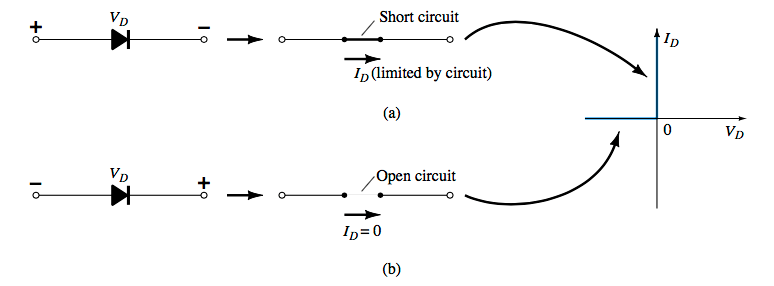
\includegraphics[height = 7cm, width = 16.5cm]{3.png}
\centering \linebreak \linebreak Figure 3.2.1: Steps to create the coding tree starting from the priority queue.
\end{figure} \hfill \break

Finally, in line 14 we store the {\itshape heap-tree} in the same class variable that we have working with. The final result should look like in Figure 3.2.2. \hfill \break

\begin{figure}[H]
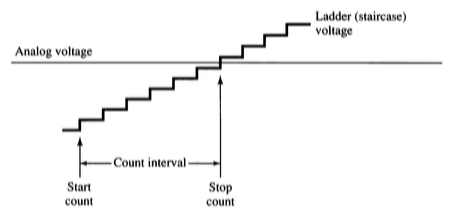
\includegraphics[height = 7cm, width = 16.5cm]{4.png}
\centering \linebreak \linebreak Figure 3.2.2: Result after combining all the nodes in the priority queue and generating a tree.
\end{figure}

\pagebreak